\documentclass{beamer}% This is the file main.tex
\usepackage{graphicx}
\usepackage{outlines}
\usepackage{gensymb}
\usepackage{tikz}


\usetheme{Boadilla}
\title{Introduction to Motor Behavior}
\author{Thad Hughes}
\date{\today}

\hypersetup{%
  colorlinks=false,% hyperlinks will be black
  linkbordercolor=red,% hyperlink borders will be red
  pdfborderstyle={/S/U/W 1}% border style will be underline of width 1pt
}

\begin{document}

\maketitle

\begin{frame}
\frametitle{Outline}
\framesubtitle{Where are we going today?}

\begin{outline}
\1 Motors, How do they work?
	\2 Brushed Motors
	\2 Brushless Motors
\1 Motor Curves
	\2 Speed vs. Torque
	\2 Power
	\2 Current
	\2 Efficiency
\1 Getting Ratio'd
\end{outline}

\begin{block}{}
	This may or may not be review for you. If it is, skim through, make sure you're comfy. If not, let this be a fun first foray!
\end{block}

\end{frame}

\begin{frame}
	\frametitle{Brushed Motors}
	
	\begin{outline}
		\1 Coils on rotor pull against magnets on housing
		\1 This rotates the rotor a little more
		\1 This makes the brushes redirect electricity into a different set of coils via the commutator
		\1 This rotates the rotor a little more, and this repeats
	\end{outline}
	\begin{columns}
	\column{0.5\textwidth}
	\begin{block}{}
	Pros: Dead-nuts simple! No fancy electronics needed.
	\end{block}
	
	\begin{block}{}
	Cons: Commutator has friction, rotor builds up heat, construction is suboptimal
	\end{block}
	\column{0.5\textwidth}
	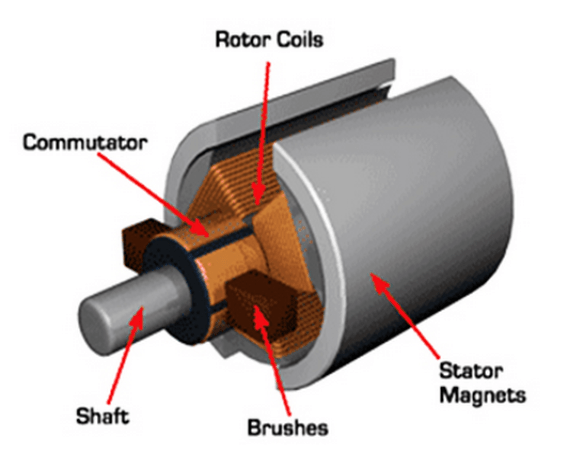
\includegraphics[width=\textwidth]{img_Mechatronics_Motors_brushed.png}
	\end{columns}
\end{frame}

\begin{frame}
	\frametitle{Brushless, Nonsensored Motors}
	
	\begin{outline}
		\1 An Electronic Speed Controller (ESC) creates an AC waveform
		\1 This waveform is fed into fixed electromagnets in the motor
		\1 This pulls and pushes the magnets on the spinning rotor
	\end{outline}
	
	\begin{columns}
	\column{0.56\textwidth}
	\begin{block}{}
	Pros: No more commutator, so higher efficiency possible. Electromagnets mounted to case, so good heat rejection.
	\end{block}
	
	\begin{block}{}
	Cons: Fancier ESC required. The AC waveform doesn't necessarially match up with the actual RPM of the motor, so best suited to low-load / high-RPM applications.
	\end{block}
	\column{0.4\textwidth}
	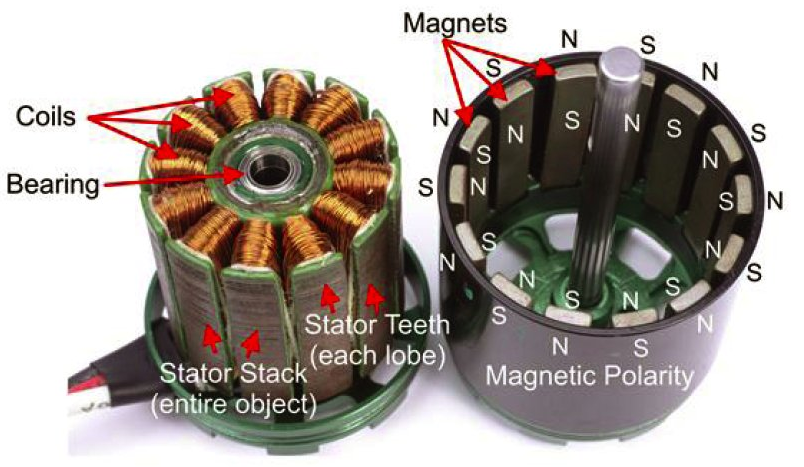
\includegraphics[width=\textwidth]{img_Mechatronics_Motors_brushless.png}
	\end{columns}
\end{frame}

\begin{frame}
	\frametitle{Brushless, Sensored Motors}
	
	\begin{outline}
		\1 Same idea as a nonsensored brushless motor
		\1 This time, though, an encoder tells the ESC where the rotor is, so the correct electromagnets can be fired, creating an AC waveform that is always in-sync with the motor's RPM
	\end{outline}
	
	\begin{block}{}
	Pros: No commutator, so high efficiency. In-sync waveform, so high torque. Builtin encoder for other applications. Maximal control over waveform possible, so highest performance. Electromagnets mounted to case, so good heat rejection.
	\end{block}
	
	\begin{block}{}
	Cons: Fanciest ESC required.
	\end{block}
\end{frame}

\begin{frame}
	\frametitle{How do these things behave?}
	\begin{outline}
\1	We usually use 'motor curves' to graph these things.
	
\1	Experimental data is very important. However, most all motors (brushed and sensored brushless) obey the same trends.
	
\1	Motor manufacturers typically provide some of these specs in some form. \href{http://motors.vex.com}{\color{red}motors.vex.com} is a very good site as well for FRC.
\end{outline}
\end{frame}

\begin{frame}
	\frametitle{Speed vs. Torque Motor Curve}
	
	\begin{columns}
	\column{0.35\textwidth}
		Torque decreases linearly with speed
		
		\begin{equation}
			T = T_{max} \frac{\omega-\omega_{max}}{\omega_{max}}
		\end{equation}
	\column{0.65\textwidth}
	\centering
	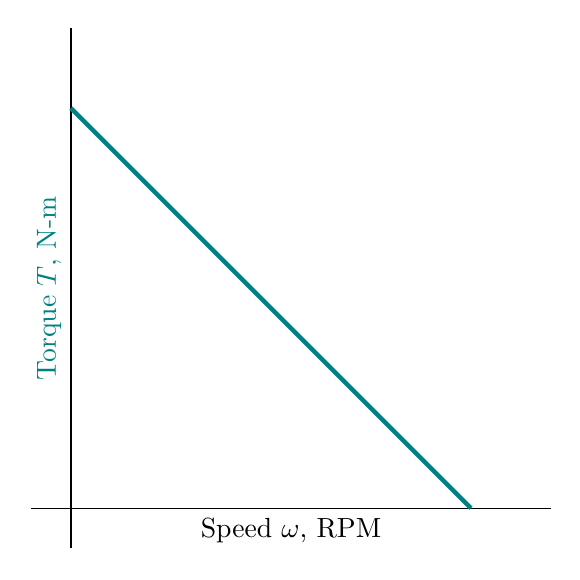
\begin{tikzpicture}[x=2.0in,y=2.0in]
		%\fill[lightgray] (1.0,0)--(0,1.0)--(0,0)--cycle;
		\draw[black] (-0.1,0)--(1.2,0) node[pos=0.5,below]{Speed $\omega$, RPM};
		\draw[black] (0,-0.1)--(0,1.2) node[pos=0.5,above,rotate=90,teal]{Torque $T$, N-m};
		
		\draw[teal, ultra thick] (1.0,0)--(0,1.0);
	\end{tikzpicture}
	
	\end{columns}
\end{frame}

\begin{frame}
	\frametitle{Power on the Curve}
	
	\begin{columns}
	\column{0.38\textwidth}
		Power is the rate at which work is done, or
		
		\begin{equation}
			P = T \cdot \omega
		\end{equation}
		
		\begin{equation}
			P = T_{max} \frac{(\omega_{max}-\omega) \omega}{\omega_{max}}
		\end{equation}
		
		\begin{alertblock}{Caveat on Calculations}
			$\omega$ must be in rad/s, not RPM.
		\end{alertblock}
		
		\begin{block}{}
			Max power occurs at 50\% speed
		\end{block}
		
	\column{0.6\textwidth}
	
	\centering
	
	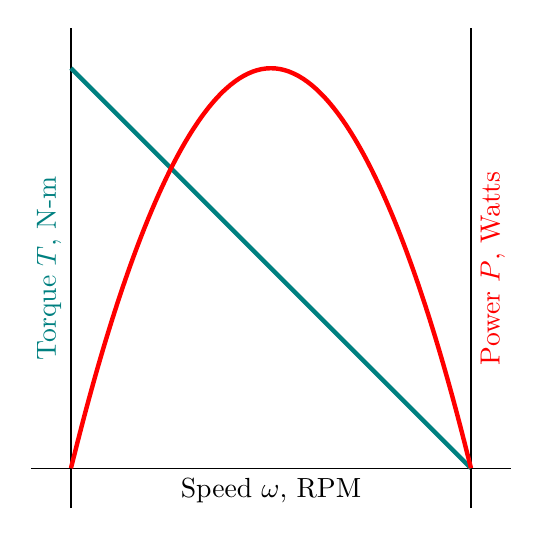
\begin{tikzpicture}[x=2.0in,y=2.0in]
		%\fill[lightgray] (1.0,0)--(0,1.0)--(0,0)--cycle;
		\draw[black] (-0.1,0)--(1.1,0) node[pos=0.5,below]{Speed $\omega$, RPM};
		\draw[black] (0,-0.1)--(0,1.1) node[pos=0.5,above,rotate=90,teal]{Torque $T$, N-m};
		\draw[black] (1,-0.1)--(1,1.1) node[pos=0.5,below,rotate=90,red]{Power $P$, Watts};
		
		\draw[teal, ultra thick] (1.0,0)--(0,1.0);
		\draw[red, ultra thick] (0,0) parabola bend (0.5,1.0) (1.0,0.0) ;
	\end{tikzpicture}
	
	\end{columns}
\end{frame}

\begin{frame}
	\frametitle{Alternate Power Visualization}
	
	\begin{columns}
	\column{0.25\textwidth}

		\begin{equation}
			P = T \cdot \omega \nonumber
		\end{equation}
		
		Power can be visualized as the rectangular area boxed in by a particular point
		
	\column{0.7\textwidth}
	
	\centering
	
	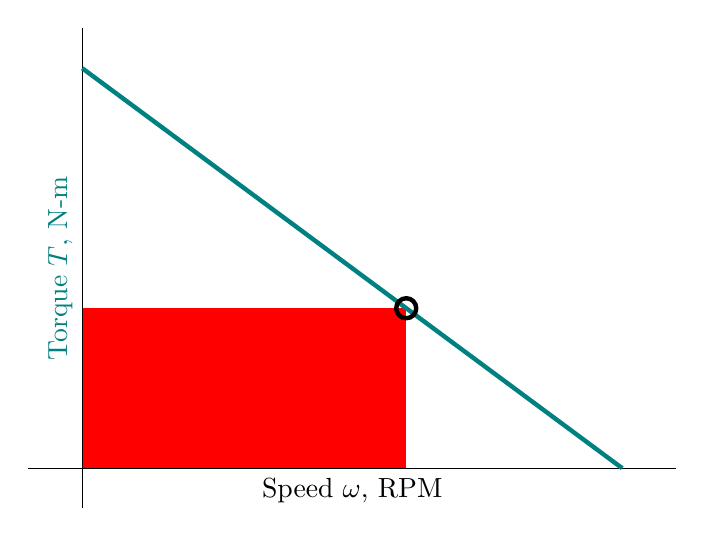
\begin{tikzpicture}[x=2.7in,y=2.0in]
		%\fill[lightgray] (1.0,0)--(0,1.0)--(0,0)--cycle;
		\fill[red] (0,0)--(0,0.4)--(0.6,0.4)--(0.6,0)--cycle;
		\draw[black] (-0.1,0)--(1.1,0) node[pos=0.5,below]{Speed $\omega$, RPM};
		\draw[black] (0,-0.1)--(0,1.1) node[pos=0.5,above,rotate=90,teal]{Torque $T$, N-m};
		%\draw[black] (1,-0.1)--(1,1.1) node[pos=0.5,below,rotate=90,red]{Power $P$, Watts};
		
		\draw[teal, ultra thick] (1.0,0)--(0,1.0);
		%\draw[red, ultra thick] (0,0) parabola bend (0.5,1.0) (1.0,0.0) ;
		
		
		\draw[black, ultra thick] (0.6,0.4) circle (0.05in);
	\end{tikzpicture}
	
	\end{columns}
\end{frame}

\begin{frame}
	\frametitle{Current on the Curve}
	
	\begin{columns}
	\column{0.38\textwidth}
		Current ($I$) is how much electricity is drawn. It varies proportionally to torque, so
		
		\begin{equation}
			I = C T
		\end{equation}		
		
		\begin{equation}
			I = C T_{max} \frac{\omega_{max}-\omega}{\omega_{max}}
		\end{equation}
		
		\begin{block}{}
			"Stall" current is the peak current, happening at 0 RPM
		\end{block}
		
	\column{0.6\textwidth}
	
	\centering
	
	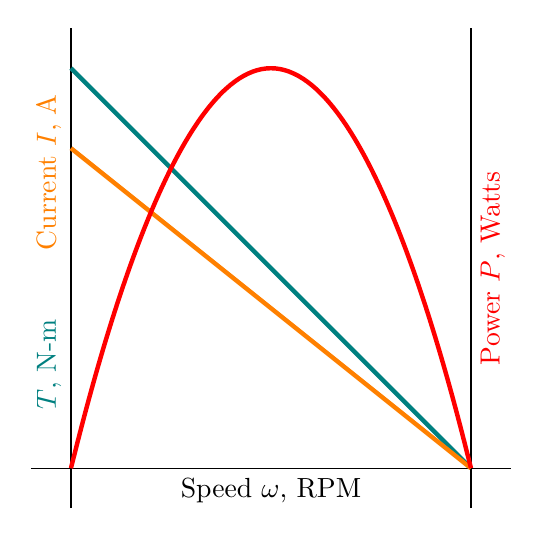
\begin{tikzpicture}[x=2.0in,y=2.0in]
		%\fill[lightgray] (1.0,0)--(0,1.0)--(0,0)--cycle;
		\draw[black] (-0.1,0)--(1.1,0) node[pos=0.5,below]{Speed $\omega$, RPM};
		\draw[black] (0,-0.1)--(0,1.1) node[pos=0.3,above,rotate=90,teal]{$T$, N-m} node[pos=0.7,above,rotate=90,orange]{Current $I$, A};
		\draw[black] (1,-0.1)--(1,1.1) node[pos=0.5,below,rotate=90,red]{Power $P$, Watts};
		
		\draw[teal, ultra thick] (1.0,0)--(0,1.0);
		\draw[orange, ultra thick] (1.0,0)--(0,0.8);
		\draw[red, ultra thick] (0,0) parabola bend (0.5,1.0) (1.0,0.0) ;
	\end{tikzpicture}
	
	\end{columns}
\end{frame}

\begin{frame}
	\frametitle{Efficiency}

		Efficiency ($\eta$) is a ratio of how much mechanical energy is produced per electrical energy spent.
		
		\begin{equation}
			\eta = \frac{P_{mech}}{P_{elec}} = \frac{(T-M_{friction} \omega}{V I}
				= \frac{[T_{max} \ \frac{(\omega_{max}-\omega)}{\omega_{max}} - M_f] \omega}{V\ C\ T_{max} \frac{(\omega_{max}-\omega)}{\omega_{max}}} \nonumber
		\end{equation}
		
		Indeed an ugly equation, let's just plot it...

\end{frame}

\begin{frame}
	\frametitle{Efficiency on the Curve}
	\centering
	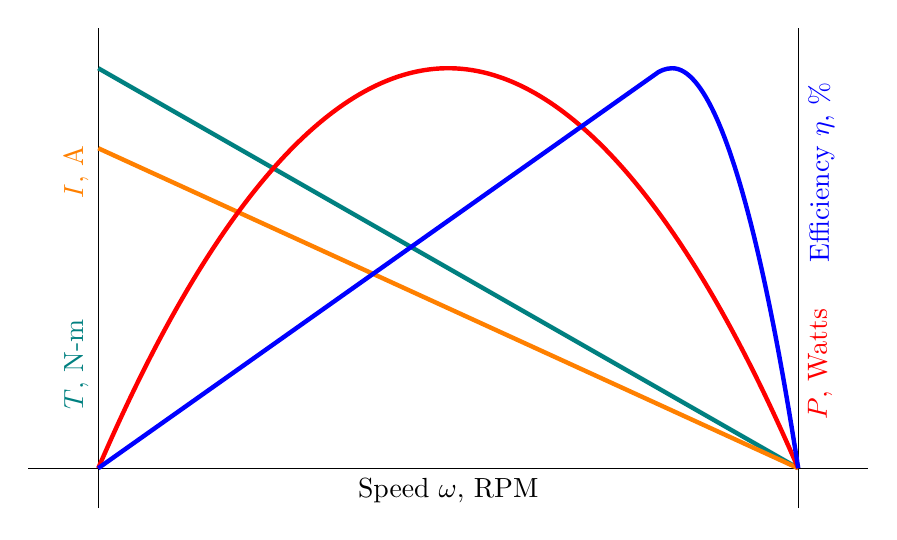
\begin{tikzpicture}[x=3.5in,y=2.0in]
		%\fill[lightgray] (1.0,0)--(0,1.0)--(0,0)--cycle;
		\draw[black] (-0.1,0)--(1.1,0) node[pos=0.5,below]{Speed $\omega$, RPM};
		\draw[black] (0,-0.1)--(0,1.1) node[pos=0.3,above,rotate=90,teal]{$T$, N-m}
			node[pos=0.7,above,rotate=90,orange]{$I$, A};
		\draw[black] (1,-0.1)--(1,1.1) node[pos=0.3,below,rotate=90,red]{$P$, Watts}
			node[pos=0.7,below,rotate=90,blue]{Efficiency $\eta$, \%};
		
		\draw[teal, ultra thick] (1.0,0)--(0,1.0);
		\draw[orange, ultra thick] (1.0,0)--(0,0.8);
		\draw[red, ultra thick] (0,0) parabola bend (0.5,1.0) (1.0,0.0) ;
		\draw[blue, ultra thick] (0,0)--(0.8,0.99) parabola bend (0.82,1.0) (1.0,0.0) ;
	\end{tikzpicture}
	\begin{block}{}
		Peak efficiency occurs usually between 75-90\% of max RPM.
	\end{block}
\end{frame}

\begin{frame}
	\frametitle{Getting Ratio'd}
	Gear ratios allow us to 'shift the curve'.
	
	If we have a motor with a pinion of $N_m$ teeth, mating with a driven gear of $N_d$ teeth, we would achieve a gear ratio of
	
	\begin{equation}
		G = \frac{N_d}{N_m} = \frac{\omega_m}{\omega_d} = \frac{T_d}{T_m}
	\end{equation}
	
	This also works with belts or sprockets and chain (though you may need to keep an eye on the direction of rotation, as gears can reverse the direction of rotation).	
\end{frame}

\begin{frame}
	\frametitle{Shifting the Curve}
	
	\centering
	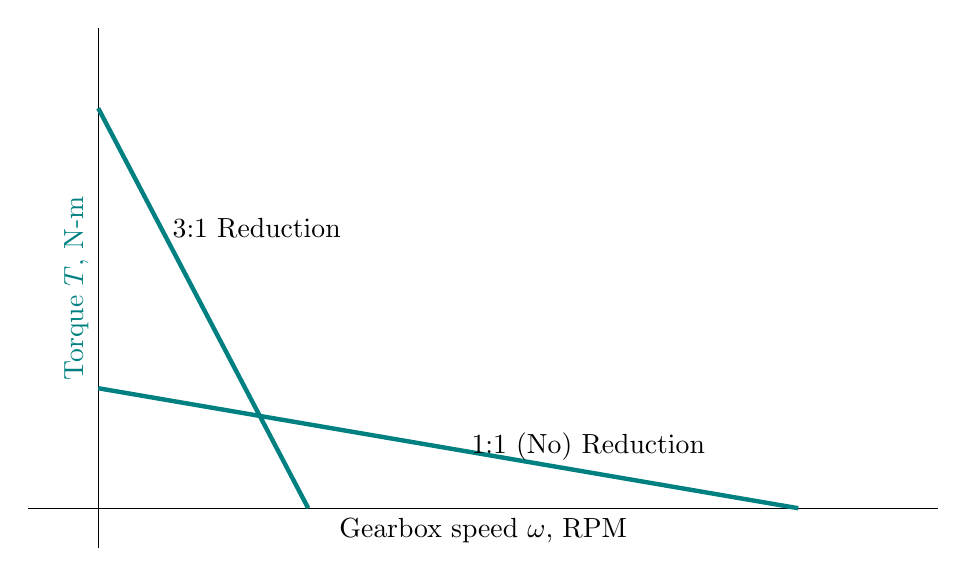
\begin{tikzpicture}[x=3.5in,y=2.0in]
		%\fill[lightgray] (1.0,0)--(0,1.0)--(0,0)--cycle;
		\draw[black] (-0.1,0)--(1.2,0) node[pos=0.5,below]{Gearbox speed $\omega$, RPM};
		\draw[black] (0,-0.1)--(0,1.2) node[pos=0.5,above,rotate=90,teal]{Torque $T$, N-m};
		
		\draw[teal, ultra thick] (1.0,0)--(0,0.3) node[pos=0.3, above, black]{1:1 (No) Reduction};
		\draw[teal, ultra thick] (0.3,0)--(0,1.0) node[pos=0.7, right, black]{3:1 Reduction};
	\end{tikzpicture}	
	
	\begin{block}{}
		The 3:1 ratio reduces maximum speed, but increases the maximum torque.
		It also changes the RPM at which maximum power and efficiency occur.
	\end{block}	
	
\end{frame}

\end{document}